%\documentclass[letter,10pt,final]{article}
\documentclass[letter,10pt]{article}
\usepackage[utf8]{inputenc}

\usepackage{listings}
\usepackage{lstautogobble}
\usepackage{textcomp}	% To get straight quotes
\usepackage[T1]{fontenc}	% To get straight double quotes
%\lstset{language=HTML}
\lstset{breaklines=true}
\lstset{showstringspaces=false}
\lstset{numbers=left}
\lstset{autogobble}
\lstset{upquote=true} % To get straight quotes
\lstset{captionpos=b} % Set caption position to bottom
%\lstset{caption=\lstname}

\usepackage{graphicx}
\setkeys{Gin}{width=.8\linewidth}

\usepackage{xcolor}
\definecolor{criticalColor}{HTML}{FF3333}
\definecolor{refinementColor}{HTML}{B3FFCC}
\definecolor{infoColor}{HTML}{FFFF80}
\usepackage[obeyFinal,color=criticalColor,figwidth=.8\textwidth]{
todonotes}
\usepackage{hyperref}
\hypersetup{
    colorlinks,
    linkcolor={red!50!black},
    citecolor={blue!50!black},
    urlcolor={blue!80!black}
} %TODO: Check colors
\usepackage{nameref}

%http://tex.stackexchange.com/questions/60209/how-to-add-an-extra-level-
%of-sections-with-headings-below-subsubsection
\makeatletter
\renewcommand\paragraph{\@startsection{paragraph}{4}{\z@}%
            {-2.5ex\@plus -1ex \@minus -.25ex}%
            {1.25ex \@plus .25ex}%
            {\normalfont\normalsize\bfseries}}
\makeatother
\setcounter{secnumdepth}{4} % how many sectioning levels to assign 
%numbers to
\setcounter{tocdepth}{4}    % how many sectioning levels to show in ToC

%opening
\title{Automating Code Magnet Generation}
\author{Julia Dana}
\date{}

\begin{document}

\maketitle

\clearpage
\tableofcontents

\clearpage
\listoftodos

\clearpage

% Defense of the choice of problem
\section{Introduction} 

\subsection{The Overview: Easier Creation of Code Magnet Microlabs}

The purpose of this project is to assist in the creation of code magnet 
microlab assignments for WAGS by creating magnets from a completed 
solution file. This is accomplished in a manner that supports multiple 
programming languages, and allows additional languages to be added with 
minimal configuration. Additional tools that support this idea of 
easier creation of assignments are also included, such as an automated
interaction with the WAGS website to create assignments. Also, this 
project defines new formats for representing magnets, both as
objects, and serialized to JSON or YAML. 

\subsection{The Context: What is WAGS?}

WAGS (Web Automated Grading System) is an ongoing project of 
Appalachian State University. It is an online tool for microlabs. 
Microlabs are short, 5-10 minutes hands-on activities that are 
intended to be done as a part of a regular (i.e. not lab) class session 
to reinforce the concepts that are currently being covered. There 
are multiple types of microlabs provided by WAGS, but the one that 
this project is interested in is code magnet microlabs. These are 
microlabs where the student is given code magnets (pieces of code). 
Then the student must choose the correct magnets to use and drag 
and drop them into the correct order to “write” a solution to the 
microlab.

\begin{figure}[h!]
 \centering
 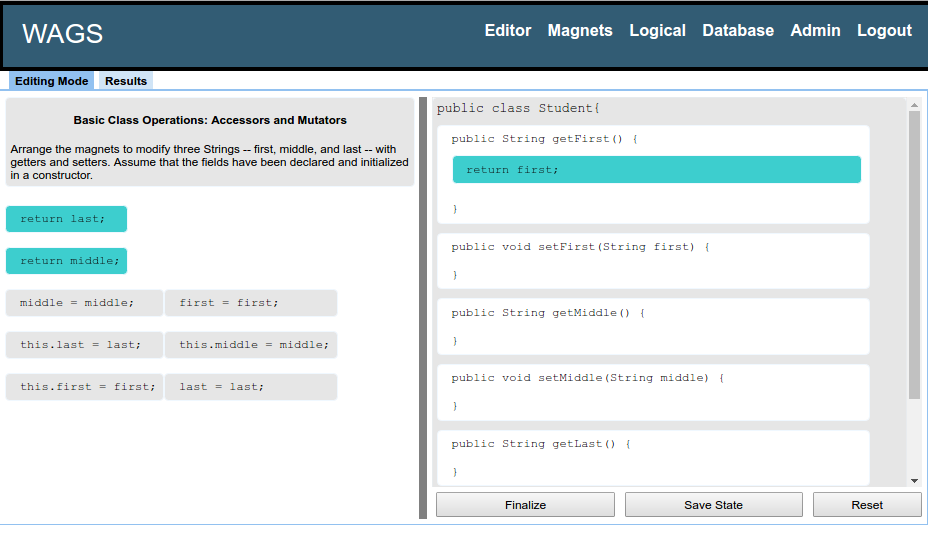
\includegraphics{./images/magnet-lab.png}
 \caption{An in-progress magnet microlab}
 \label{fig:magnet-lab}
\end{figure}

\subsection{The Problem: Brittle Input}

The problem is that creating these magnet microlab assignments on the 
WAGS website is a somewhat painful process. The current parser creates 
magnets based on whitespace (line breaks and indentation). This limits 
the style of code that can be used. For example, opening curly braces 
in Java must be on the same line as the class/method/loop they are 
associated with. Also, statements have to be on a single line, 
regardless of length. See Figure \ref{fig:old_parser_style} for an 
example \cite{icer_pres_4_creating_lab}. These sylistic limitations, 
while limiting, do not force your input to the microlab creation to 
become an invalid solution file. However, to create alternative magnets 
for the existing parser, one adds extra lines to the input file. This 
does change the input file to no longer be a correct solution, and can 
even change it to no longer be a valid file for its language. This 
means that the instructor now has to maintain and keep in sync both a 
proper solution and the WAGS input file. See Figure 
\ref{fig:old_parser_alts} to see how adding alternative magnets 
can change an input file\cite{icer_pres_4_creating_lab}.

\begin{figure}[h!]
 \centering
 
  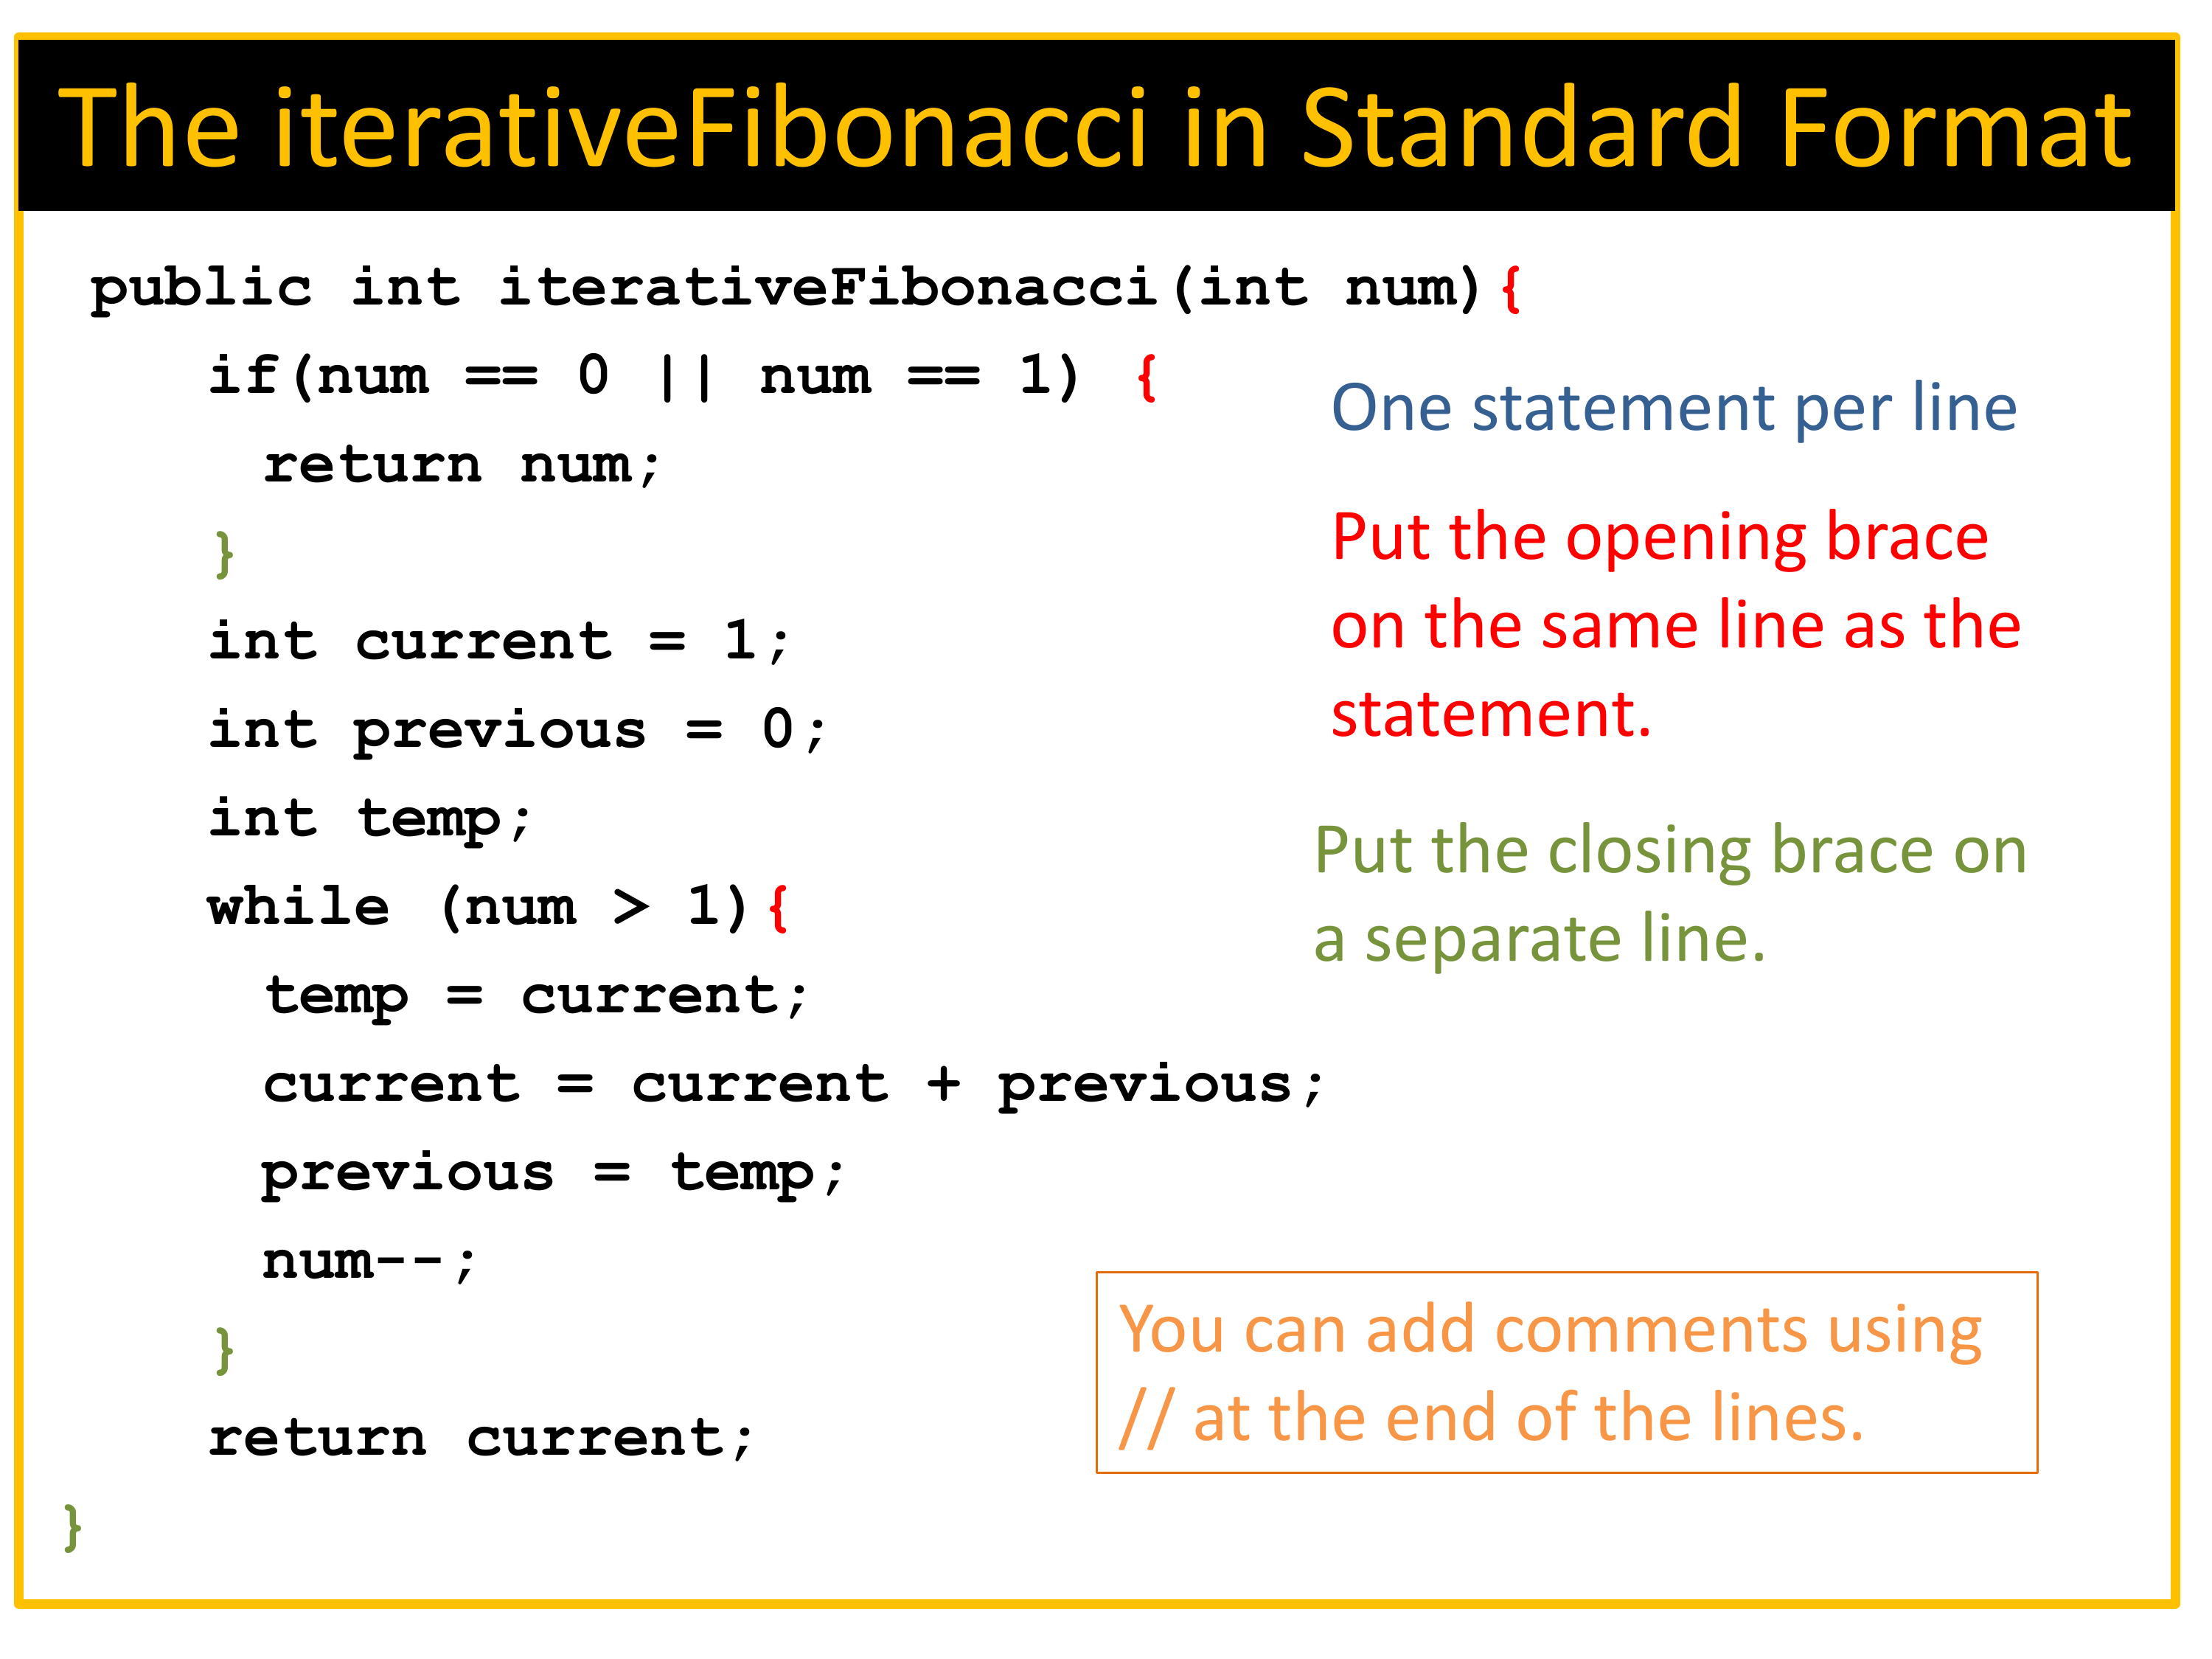
\includegraphics{%    
./images/CreatingCodeMagnetLab/old_parser_presentation-07.png}
 \caption{Putting an Input File In Standard Format}
 \label{fig:old_parser_style}
\end{figure}

\begin{figure}[h!]
 \centering
 
 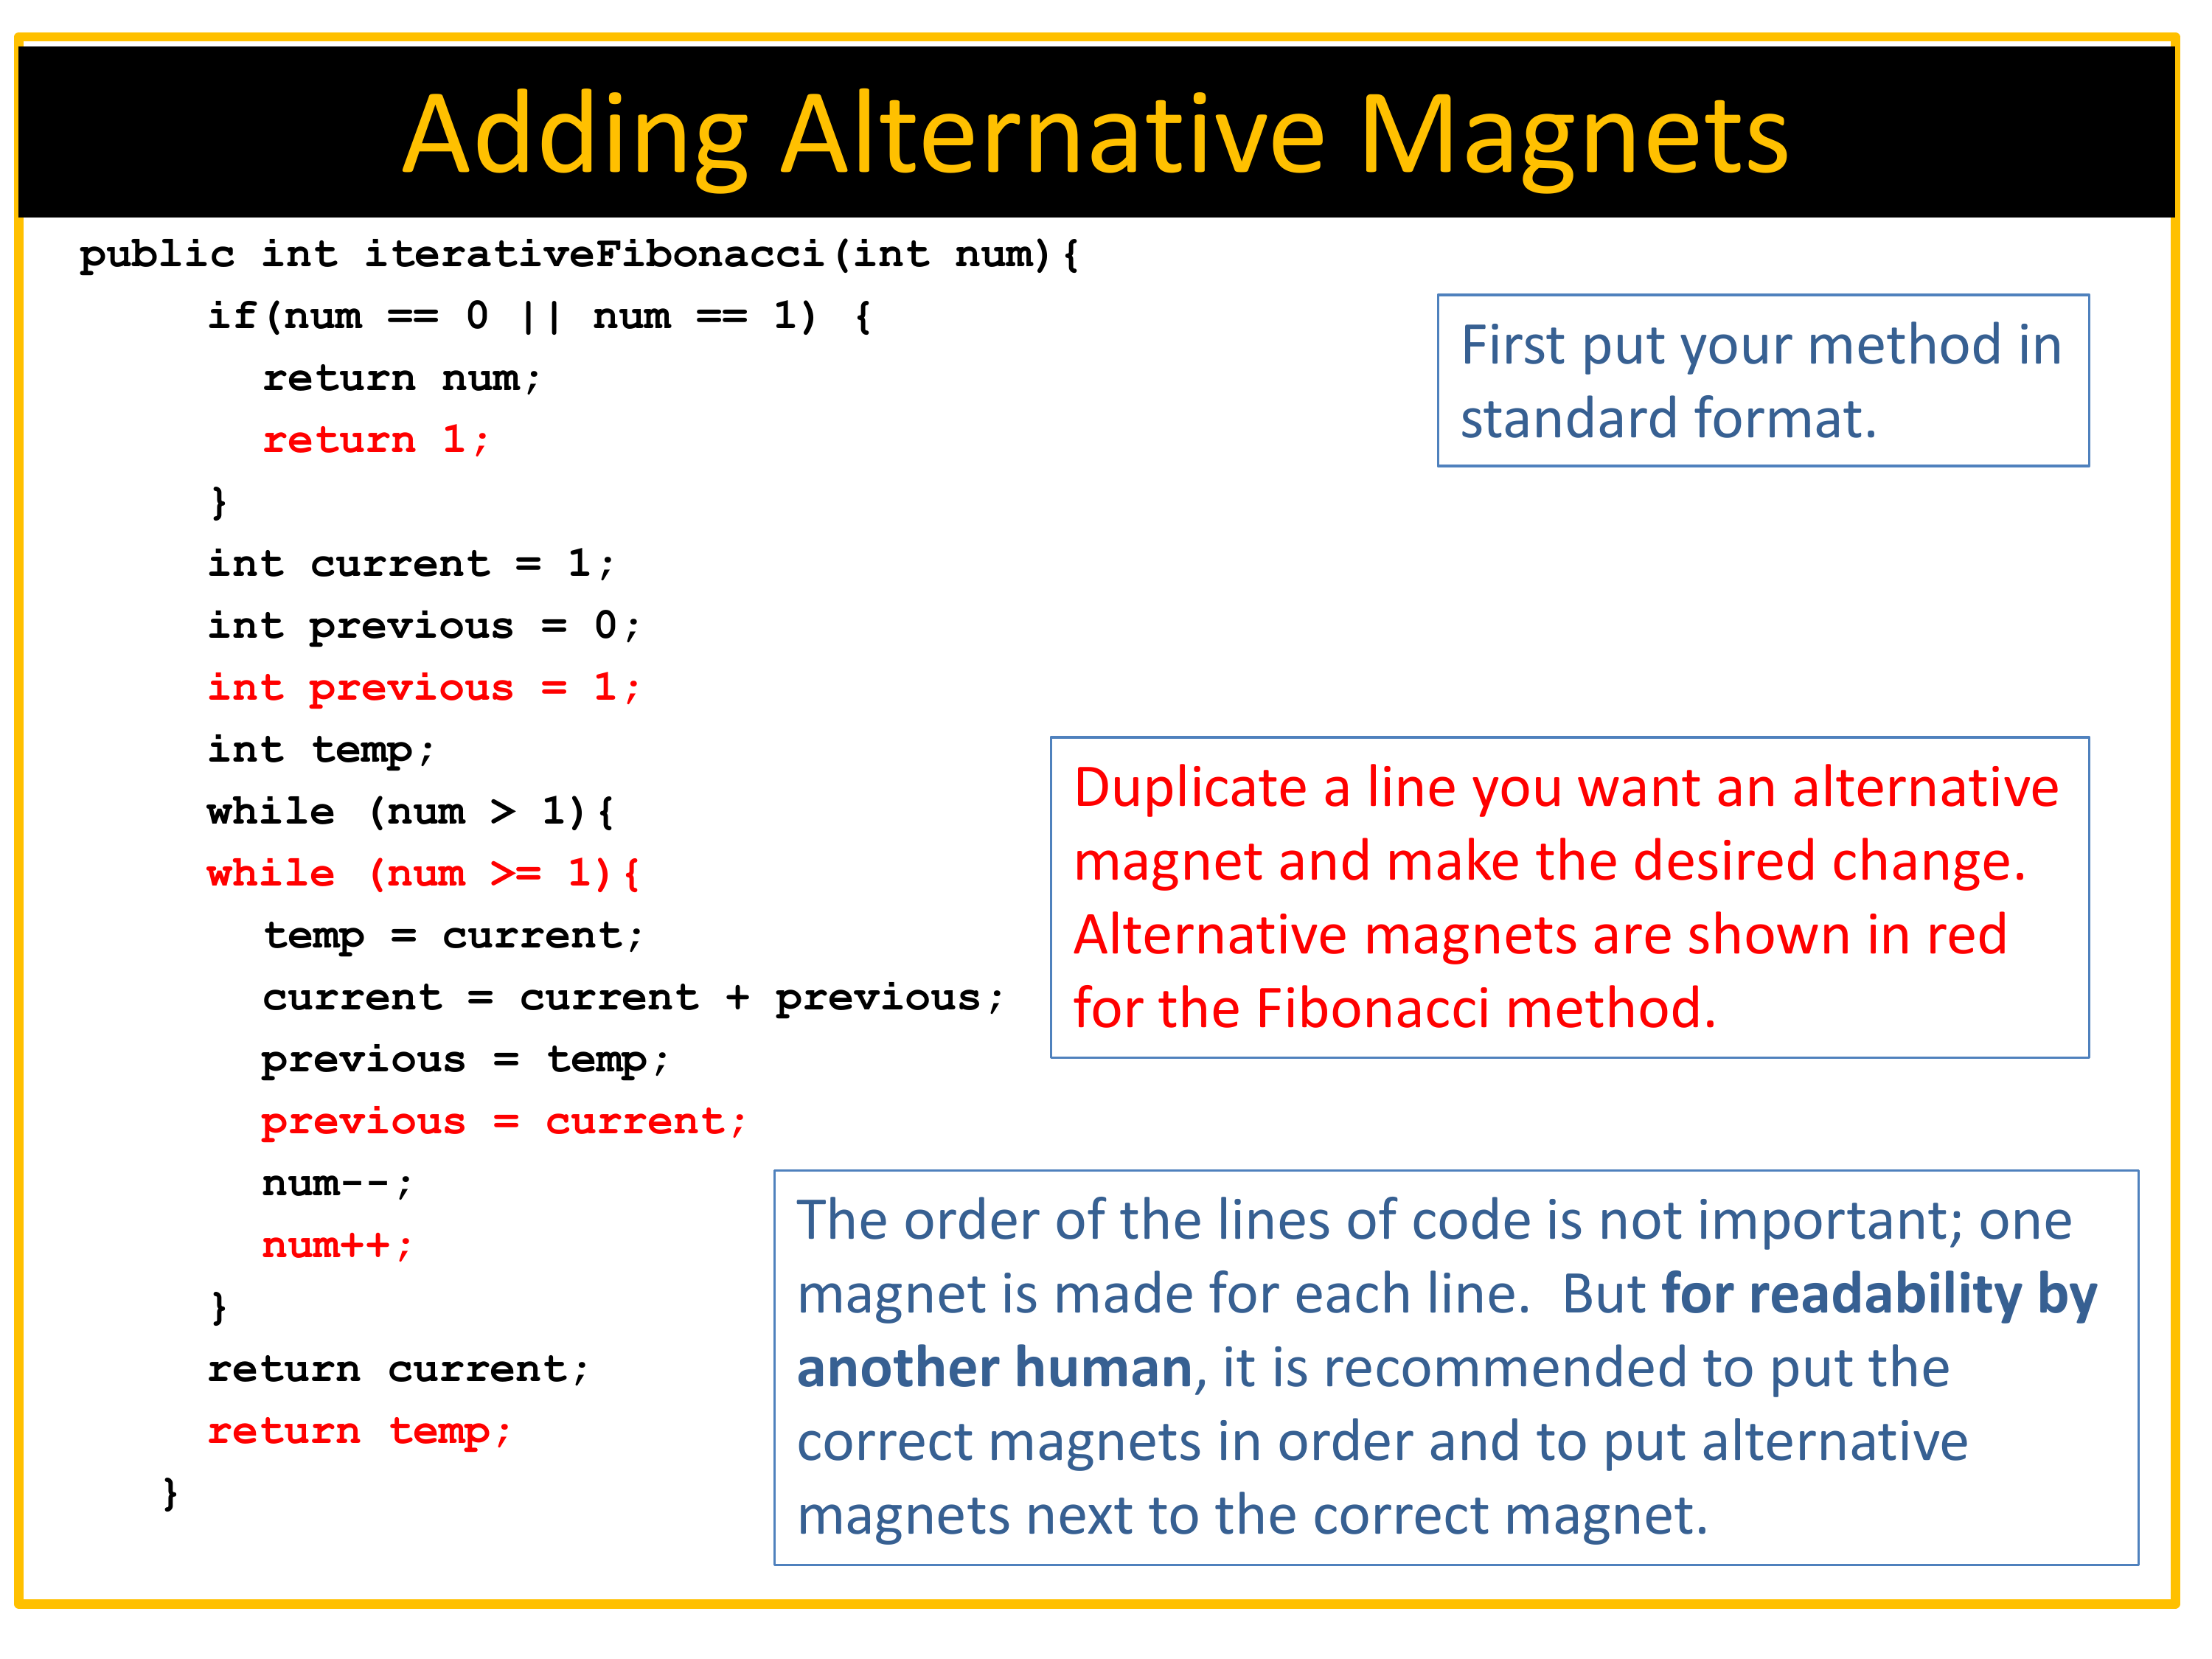
\includegraphics{%
./images/CreatingCodeMagnetLab/old_parser_presentation-09.png}
 \caption{Adding Alternative Magnets}
 \label{fig:old_parser_alts}
\end{figure}

If your input cannot be handled by this brittle parser. WAGS does 
provide a manual input for magnets. However, using this manual input 
requires magnets to either be entered one at a time to the magnet 
creation wizard, or for the user to directly type the final magnet 
(including HTML escape sequences) to the parsed output section. 

\begin{figure}[h!]
 \centering
 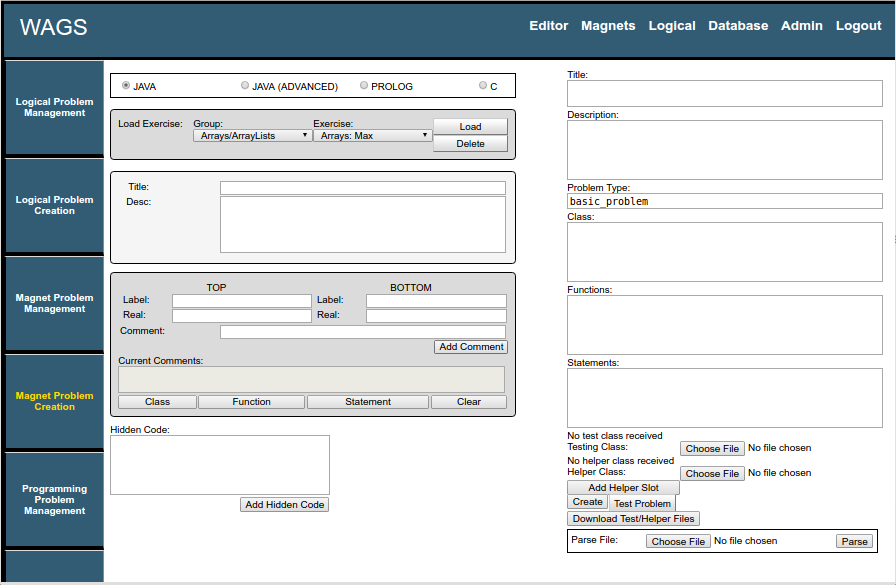
\includegraphics{./images/wags-magnet-creation.png}
 \caption{WAGS Magnet Assignment Creation Page}
 \label{fig:wags-magnet-creation}
\end{figure}


\subsection{The Solution: Parsing by Grammar}

The solution to the problems raised by the old, brittle parser is to 
use a more robust parser that is based on the grammar of the language, 
rather than the formatting of the input file. This project does this by 
using the ANTLR4 parser generator\cite{antlr-reference} and freely 
available grammars for common languages\cite{antlr-grammars-project}.

A grammar is a formal specification of a language. It is a series of 
rules (called productions) that define valid phrases of a language. A 
single production could define the structure of an entire file, or just 
be a single statement or expression. A production is the valid 
components of a statement (tokens and other rules). A rule can match 
one or more productions.

There are many parallels between a grammar of a programming language, 
and the grammar of a natural language (such as English). 
As a rough comparison, using a grammar-based parser to 
break code into magnets is like breaking apart a paragraph based on 
sentences or phrases, rather than on every period (Which commonly 
indicates the end of a sentence, but also has other uses, such as 
abbreviations). This type of parser will create tokens from the input, 
which are loosely the equivalent of words, and then break them into 
(sometimes nested) phrases and sentences according to rules called 
productions. Rules are named, and will sometimes contain more than one 
production as alternatives that provide the same function in a 
language. 

A parser uses these rules to build a parse tree. The root of the parse 
tree is the start rule. The interior nodes of the parse tree are rules 
from the grammar. The leaf nodes of the parse tree are tokens from the 
lexer.

This project specifies which rules in the grammar should create their 
own magnets. If a rule is nested in another rule only the magnet of the 
nested rule gets the text. The magnet for the outer rule replaces the 
text of the nested rule with a drop zone (an area that accepts magnets)

Using a parsed file gives us a high level of control over how and when
to create magnets. However, writing a robust parser is a non-trivial 
task. Today, most parsers are created by parser generators. These take 
the description of the language given in a grammar, and creates the 
parser for that language. There are many such parser generators, 
including YACC \cite{yacc_homepage}, Bison \cite{bison_homepage}, and 
CUP \cite{cup_homepage}. This project uses the ANTLR4 
\cite{antlr_homepage} parser generator, which generates parsers in 
Java. 

\todo[color=refinementColor]{expand on ANTLR - LL(star) - other 
features} 

% Defense of solution
\section{Development results and future extensions}

\subsection{What It Does: Internal Functions}

\subsubsection{Parses by Grammar}

The magnetizer takes an input file, and parses it with the parser 
generated by ANTLR from the grammar specification. The result of this 
parsing is a parse tree, which is then used to create magnets. ANTLR 
can show us a graphical representation of this tree, as follows.

For this simple Java file, Hello.java
\lstinputlisting[language=Java, caption={Hello.java}]{./code/Hello.java}

The resulting parse tree is:

\begin{figure}[h!]
 \centering
 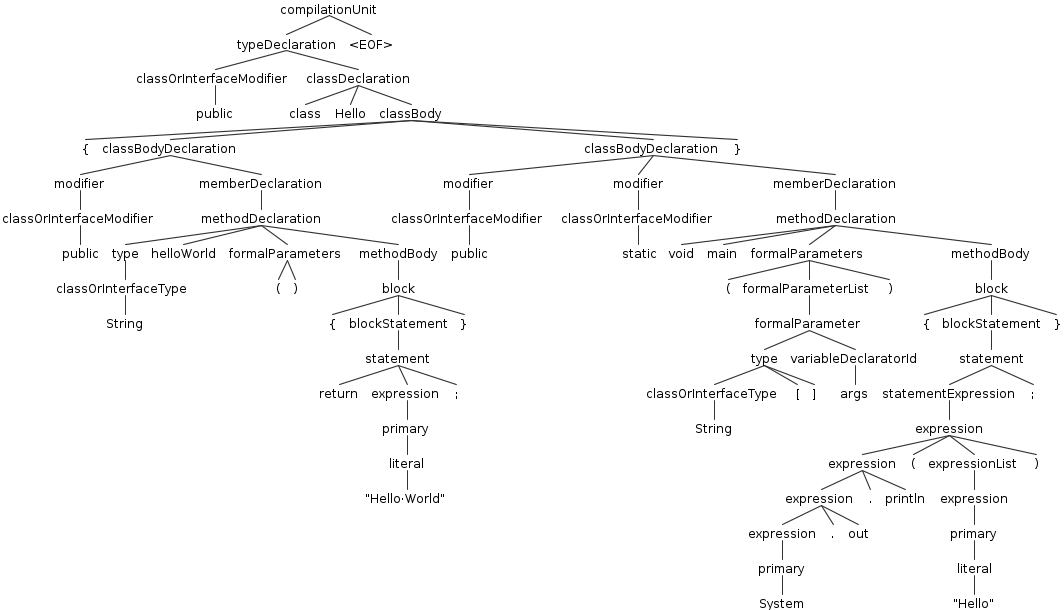
\includegraphics[width=\linewidth]{./images/hello_parse_tree.png}
 \caption{The parse tree from Hello.java}
 \label{fig:hello_parse_tree}
\end{figure}

ANTLR provides two mechanisms for traversing this tree once it is 
created. One is a walker, which triggers enter and exit methods in a 
listener for each type of internal node, and the other is a visitor, 
which has methods for visiting each type of internal node. For 
both mechanisms, ANTLR provides a Java class which is a base version of 
the listener or visitor, with stubs of the methods containing minimal 
functionality. The programmer can then subclass these base 
versions to perform their project-specific actions at certain nodes. 
This project initially used the listener mechanism, but later switched 
to using the visitor to make it easier to implement the NODROP 
instructor directive. One key difference between the mechanisms is that 
the walker/listener method will always visit every node in the tree. 
With the visitor method, the base (ANTLR-generated) visitor visits 
every node by default, but the specific visitor can choose to not visit 
some or all of the children of a node, because the visit method is 
responsible for chosing when to visit children.

The visitors for this project are dynamically created JRuby subclasses 
of the ANTLR-generated base visitors. There is an ANTLR-generated base 
visitor per supported language. There is a single JRuby generator that 
creates a subclass of the Java base visitor for any language. The 
generation of the subclass is controlled by an entry in a configuration 
file which specifies the name of the grammar used (language name), and 
which rules (which become internal nodes in the parse tree) trigger the 
creation of a magnet. This dynamic generation prevents repeated code 
because we want to perform the same types of actions at every node that 
triggers a magnet, but the structure that ANTLR expects requires 
separate methods.

\lstinputlisting[caption={The section of the configuration file that 
sets up Java magnetization}]{./code/java_config.yaml}

\todo{Show subclass generating code}

One difficulties encountered in creating magnets from the parse tree 
is that the ANTLR-generated parser (like most parsers) discards 
whitespace once the parse tree has been built. By default, only the 
tokens themselves are kept. So, although the nodes in the tree 
provide a getText() method, the result of this is something 
like \verb~publicclassMyClass~ rather than the expected 
\verb~public class MyClass~. However, ANTLR provides a way to keep extra
information such as whitespace and comments around for later use if they 
are needed called hidden channels \ref{fig:channels}. This splits the 
incoming token stream into a channel for use by the parser, and hidden 
channels that can later be accessed to recreate the original text (with 
formatting) for the magnet. This hidden channel mechanism is also used 
to implement instructor directives.

\begin{figure}
 \centering
 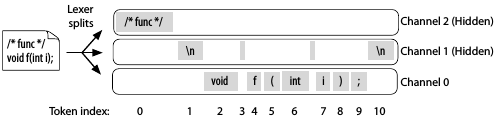
\includegraphics{./images/antlr-hidden-channels.png}
 \caption{Diagram of tokens being split into %
channel\cite[207]{antlr-reference}}
 \label{fig:channels}
\end{figure}



\subsubsection{Alternative Magnets and Other Instructor Directives}

Instructor directives allow instructors to control how magnets are 
created. They are implemented as special comments that go to a 
special token channel. The content of directives are the same across all 
languages, but the triggering comment syntax is specific to each input 
language. Current directives implemented all instructors to suppress 
drop zones (NODROP), to indicate that a duplicate magnet with a section 
of alternate text should be created (ALT and ENDALT), and to create an 
unrelated magnet (EXTRAMAG).

\todo{Discuss limitations in Python due to Indent/Dedent tokens}
All the directives currently work with Java input file. However, there 
are some limitations with directives in Python. Because comments in 
Python always go to the end of a line, creating a magnet with alternate 
text does not work, since the original text cannot be surrounded by 
comments. Also because of line-based comments, unrelated magnets must 
be created in a single line. There are also some cases where directives 
do not properly get connected to the expected node in the tree because 
indentation is not considered discardable whitespace in Python.

\subsubsection{Improved Representation of Magnets}

The old format for describing magnets is difficult to read and worse to 
try to manually type. Some of its quirks are that magnets are separated 
by an unusual separator (\verb~.:|:.~), areas that accept other magnets 
(aka drop zones) are indicated by a seemingly random set of HTML tags 
(\verb~<br><!-- panel --><br>~), and any special characters used in the 
code magnet must be escaped for HTML (so something like \verb~1 < 2~ 
would need to be entered as \verb~1 &lt; 2~). This format also is 
limited when trying to create more advanced types of magnets. The WAGS 
system addresses this problem by adding more form fields when adding 
``advanced Java magnets'', but this does not work well for adding 
additional languages.

\begin{figure}[h!]
 \centering
 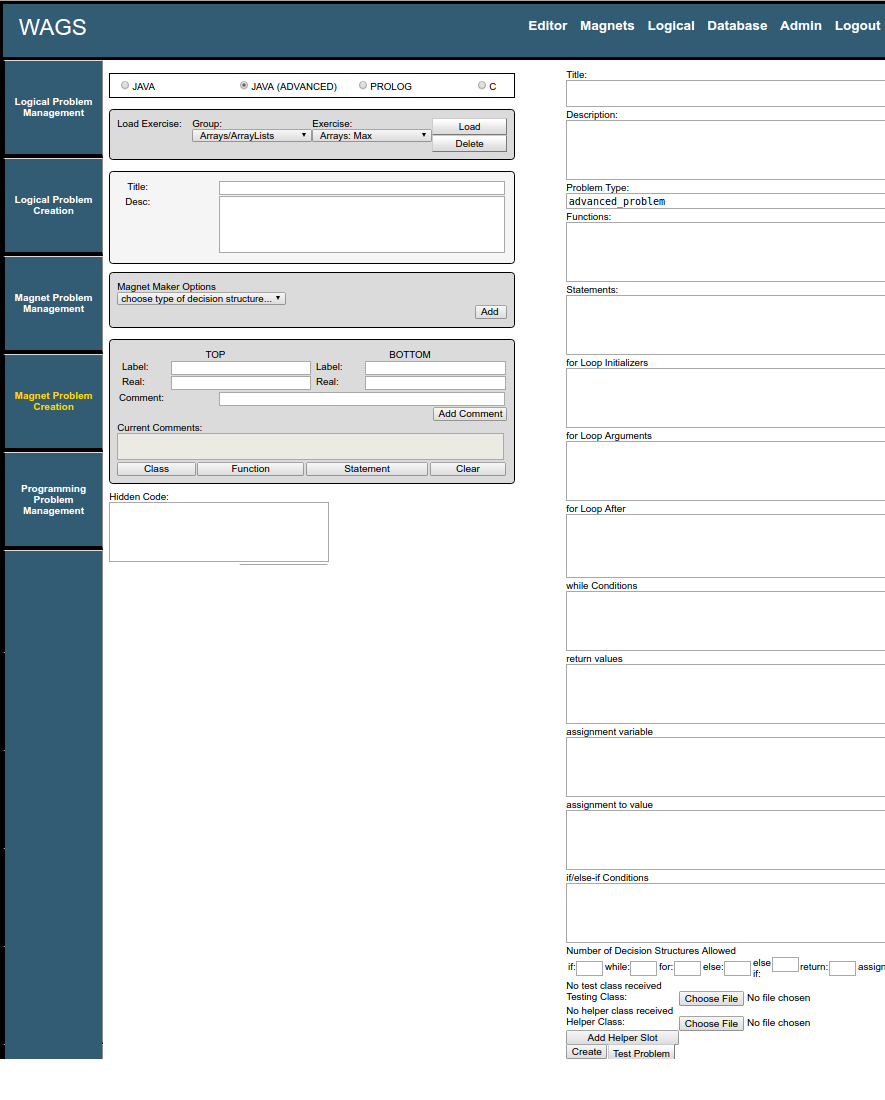
\includegraphics{./images/wags-adv-magnet-creation.png}
 \caption{Creating a magnet assignment with advanced magnets}
 \label{fig:wags-adv-magnet-creation}
\end{figure}


This project creates an underlying object based data structure for 
magnets, as shown in figure \cite{fig:magnet-diagram}. This structure 
can then be serialized as desired. Currently, serialization to the old 
magnet format is supported for backward compatibility, as well as JSON 
and YAML for more robust usages.

\begin{figure}[h!]
 \centering
 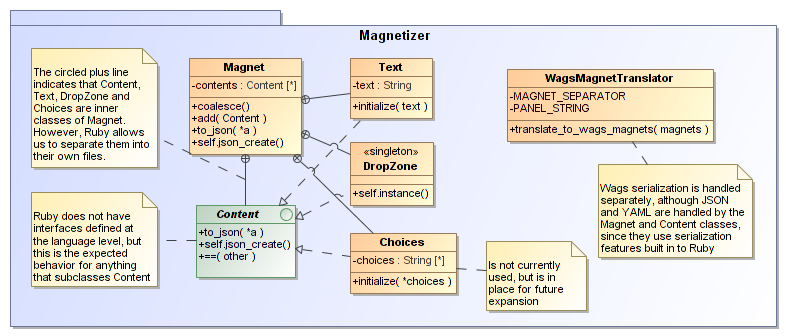
\includegraphics[width=.95\linewidth]{%
./images/FinalMagnetStructure.png}
 \caption{The classes of the magnet data structure}
 \label{fig:magnet-diagram}
\end{figure}



\subsection{What It Does: External Functions}

\subsubsection{Command Line Tool}

This project provides a command line tool, which is a thin wrapper 
exposing the internal API functions to the command line.


\subsubsection{Automated Interaction With WAGS Website}

This project contains a proof-of-concept automated interaction with the 
WAGS website, which is capable of logging in to the site, and creating 
an assignment with magnets from a specified input file. The assignment 
that is created has the magnets loaded, but it does not have any of the 
other files that the WAGS system needs to automatically provide 
feedback to the students. The automated interaction is provided using 
libraries commonly used in Ruby for automated testing of websites. It 
uses the Capybara acceptance test framework (which provides a 
convienient, cross web driver DSL for interacting with websites), the 
Poltergeist web driver, and the PhantomJS headless browser. Support for 
Capybara, the Selenium web driver, and Firefox browser is coded, but 
Selenium will not trigger the log in button on the current web site.


\subsection{What It Could Do: Future Extensions}

\subsubsection{Automatic Generation of Alternative/Distractor Magnets}

The next step in easily creating code magnet assignments is to have the 
magnet creation tool not simply create magnets needed for the correct 
solution and any additional magnets specified by the instructor, but 
also to automatically create appropriate alternative ``distractor'' 
magnets for common student misconceptions and errors. This level of 
manipulation is available because we have the whole parse tree to work 
with during magnet creation, but would require significant work per 
language to define.

\subsubsection{GUI Tool}

A GUI tool that can open an input file, perform the actions of the CLI 
tool on it, and also has an editor to assist in the addition of any 
instructor directives desired would be a nice addition to this project.

\subsubsection{Further Automated Interaction With WAGS Website}
It would be nice if this project could completely and reliably upload 
new magnet assignments to the WAGS website. The current interaction 
with the website does not upload the test file or any information other 
than the magnets. It also does not support the advanced Java magnet 
upload page. It also only works with the headless web driver 
(Poltergeist), not the one that shows the user what is happening 
(Selenium). However the limiting factor is that the functionality of 
the WAGS site is split between two versions of the website, and that 
the site has not been designed with programmatic interaction in mind.

\subsubsection{Supporting New Languages}

This project currently can create magnets for Python3 and Java, however 
it is set up to easily allow the addition of new languages. 
Basically, this is done by finding and adding an ANTLR4 grammar file 
for the desired language, making sure it conforms to a handful of 
guidelines, writing a short configuration file, and running a setup 
action on the project. Full details of this process are in 
section~\ref{sec:newLang} \nameref{sec:newLang}.


\subsubsection{Additional Serialization Formats}

Because magnets are now objects, additional serialization formats (such 
as XML) could easily be added. 



% Targeted to a CIS 1 instructor
\section{User Guide}

\subsection{Quick Start - CLI Tool}

The primary interface to this project is the magnetizer command line 
tool.  This tool is packaged as a stand-alone executable JAR file. 

It takes as input a file name, and outputs the magnets created 
from the input file. By default it assumes the input file is in Java. 
If it is in Python, the language options needs to be specified as 
Python3. 

By default, it prints the magnets in WAGS format to the console. It can 
also or instead print the magnets to JSON or YAML. It also can 
send the magnets to a specified output file, rather than the console. 

\begin{verbatim}
Usage: magnetizer [options] file
    -l, --language LANGUAGE          Specify a language (default: Java, 
                                       other: Python3)
        --json                       Print the JSON output
        --yaml                       Print the YAML output
        --[no-]wags                  Print the output as WAGS magnets 
(default)
    -o, --output-file BASE_FILENAME  Output to a file
    -h, --help                       Show this message
\end{verbatim}


\subsection{Installation for Use}
This tool is packaged as a stand-alone JAR file. It does not need to be 
installed before running. Its only dependency is that Java needs to be 
installed, and it has been tested with Java ?? \todo{test Java versions}

% An overview of how a file is split into magnets.
\subsection{Explanation of Magnet Creation}

\todo{explain these in a way that doesn't require 
deep understanding of the ANTLR grammar.}

\subsubsection{Java}
The current configuration for Java creates magnets for
\begin{itemize}
 \item Package declarations
 \item Import declarations
 \item Type declarations
 \item Class body declarations - this is the nonterminal that includes 
anything that can be directly in the class body
 \item Block statements - this is the nonterminal that includes 
anything that can be directly inside a block.
\end{itemize}

\subsubsection{Python 3}
The current configuration for Python creates magnets for
\begin{itemize}
 \item simple statements
 \item compound statements
\end{itemize}


\subsection{Modifying the Magnet Creation: Instructor Directives}
Instructor directives are information that can be put in the input file 
that change how the magnets are created. They are a special version of 
comments. The triggering syntax varies per language, but the directives 
are the same for all languages.

\begin{description}
 \item [Java] \verb~ /*# <directive> */~
 \item [Python3] \verb~ ## <directive>~
\end{description}



Note that directives in python are somewhat limited because comments 
cannot occur in a line. \todo{Verify that there are no inline comments 
in python}
\todo{explain which directives work in python}

\subsubsection{ALT and ENDALT: Creating Alternative Magnets}

The ALT and ENDALT directives are used to create alternatives with 
different text for a magnet. The ALT directive also takes the desired 
alternative text, and the ENDALT directive is used to indicate where 
the end of the alternative text is. These directives should always be 
used as a pair, and encompass the text that should be replaced. They 
cannot go around anything that would trigger the creation of a new 
magnet or drop zone. This directive has only been tested in 
Java. \todo{Check state of ALT directive in Python} 

\todo{Concrete example of ALT}
Example: To provide an alternative condition for a loop in Java.

\begin{lstlisting}[language=Java]
while(/*# ALT altCondition */ realCondition /*# ENDALT */) 
{
  System.out.println("Hello");
}
\end{lstlisting}


\subsubsection{NODROP: Suppressing Drop Zones}

The NODROP directive suppresses the creation of drop zones for the 
following magnet. An example of when this would be used is to put an 
entire loop on a single magnet, rather than having the individual 
statements in the body be on their own magnets. This directive has only 
been tested in Java.\todo{Check state of NODROP directive in Python} 

\todo{Concrete example of NODROP}
Example: To create a loop whose body is contained on the main magnet in 
Java. Used when creating the body of a loop/method/etc. is not the 
focus of the microlab.

\begin{lstlisting}[language=Java]
/*# NODROP */
for (int i = 0; i < 10; i++) {
  System.out.println(i);
}
\end{lstlisting}

\subsubsection{EXTRAMAG: Creating an Extra Magnet}

The EXTRAMAG directive is used to add a magnet that is unrelated to any 
of the magnets in the input file. This directive is tested in Java and 
Python. \todo{Check state of EXTRAMAG directive in Python} 

\todo{Concrete example of EXTRAMAG}


\section{Developer Notes}
\todo[color=infoColor]{Targeted to someone expanding on this project}

\subsection{The Environment: Languages and Libraries Used}

\todo{Section needs more details}

This project is written in Ruby for the JRuby interpreter. JRuby is able
to access Java classes from Ruby. For this project, this means we can 
use to use a parser generated by ANTLR from Ruby.

Automated interaction with the WAGS site is provided by using Capybara 
to interact with Selenium (drives Firefox) or Poltergeist/PhantomJS 
(headless).

Rake (Ruby make) is used to process new grammar files and other build 
tool functionality.

RSpec is used to handle testing.

\subsubsection{Installation for Development}
\todo{Consider if this section should be on its own}

\subsection{The Design}

\subsubsection{Directory Structure}
\begin{description}
 \item [/bin]
    Contains the Ruby script that has set up as an 
executable and is the command line interface.

 \item [/data]
    Contains grammar files and language-specific 
configuration information. This is the only location that has 
language-specific information.

 \item [/doc]
    Contains documentation for the project.
    
 \item [/etc]
    Contains any external projects and libraries needed for this 
project that are not available as Ruby gems.

 \item [/java]
    Contains Java code generated by ANTLR and the compiled class files 
from that generated Java code.

 \item [/lib]
    The primary directory of the project. This contains the Ruby code 
for the magnetizer.

 \item [/spec]
    The second of the two folders used for testing. This is for RSpec 
spec tests.

\end{description}


\subsubsection{JRuby / Java Integration}

\subsubsection{Key Classes}

\begin{description}
 \item [MagnetEmitterBase] A mix-in that contains methods that have the 
same implementation across all the ruby-generated Visitors. In Ruby, a 
mix-in is a module that provides similar functionality to an abstract 
class in Java. When a class ``include''s a module as a mix-in, that 
class gets all the methods defined in that module. Unlike abstract 
classes in Java, a class can have multiple modules mixed in, and a 
mix-in is unable to define abstract methods (Ruby does not have an 
equivalent to abstract methods).

\item[MagnetEmitterVisitorGenerator] Creates the correct subclasses of 
the ANTLR BaseVisitor. This class is where the bridging magic of JRuby 
is the most obvious, because we are creating subclasses of a Java class 
in Ruby.

ANTLR provides two primary patterns for traversing a parser tree: 
listener and visitor. This project uses the visitor pattern so that we 
do not have to visit child nodes in the parse tree for nodes that we 
know are terminal to our magnet generation. 

\end{description}


\subsection{The Testing}

\subsection{The Configuration: Specifying Magnet Sections}
\label{sec:newConfig}

The configuration that handles specifying how the parse tree for a 
language should be converted to magnets. The configuration is loaded 
from a YAML file in the \verb~/data~ directory. A language 
configuration contains the name (which corresponds to the 
name of the grammar file), the name of the rule that is the start rule 
for the parsing, whether or not the language should have a file-level 
drop zone, information about the special comment that indicates 
directives for that language. The names of the rules that indicate are 
listed by which WAGS section the magnets will need to go into. There is 
also a section to specify overrides for cases where the name of the 
rule is not sufficient information, and there needs to be additional 
information used to determine which list a magnet should go in.

This YAML file describes instances of LanguageConfig class, and the 
magnetizer then uses the LanguageConfig objects to create the magnets.

\missingfigure{Link in the source code for the Java language 
specification}

\missingfigure{Class diagram of LanguageConfig, maybe?}

\subsection{The Expansion: Adding a New Language}
\label{sec:newLang}

To add a new language to be magnetized, a new grammar needs to be 
added, the project rebuilt to include that grammar, and a new 
configuration as mentioned in section~\ref{sec:newConfig} 
\nameref{sec:newConfig} needs to be added. The build file (Rakefile) 
also provides some additional tools that are helpful to visualize the 
new grammar when writing the configuration.

\subsubsection{New Grammar Specification}
A new G4 file can be added to the system. However, whitespace is
require to go on channel 1, or your magnets will not have any
whitespace, and you might get things like ``publicclassMyClass''. Also, 
special comments for the directives need to be defined, and they need 
to go on channel 2. The entire comment for a directive should be 
recognized as a single token.

\subsubsection{Rakefile: Useful Actions for Adding a New Language}

%\clearpage
%\section{Glossary}
%\todo{Write the glossary}
%\begin{description}
% \item [magnet] What a magnet is.
%\end{description}


\clearpage
\todo{Final export of bibliography from Mendeley and link it}
\todo{Make sure citations and bibliography are styled correctly}
\addcontentsline{toc}{section}{References}
\bibliography{bibliography}{}
\bibliographystyle{plain}

\end{document}
